\part{Cours Magistral 4 -- Les intégrales}
\section{Rappel}

Nous considérons deux champs de vecteurs bidimensionnels (également appelés champs vectoriels plans)
\[
\left\{
\begin{array}{c}
F=y^2\xunit+2xy\yunit\\
F = y\xunit-x\yunit
\end{array}
\right.
\]

\[\int_C F\cdot \dif r \]

\section{Intégrale le long d'un chemin}
Cette section se réfère à la section~15.4 de~\cite{adams2013calculus}

\subsection{Champ de vecteurs conservatif ou dérivant d'un potentiel scalaire}

\[F:(F_1,F_2,...F_n)\text{dans } \mathbb{R}^n\]

\[F_i=F_i(x_1,x_2,...,x_n)\]

$F$ est conservatif ssi il existe un champ scalaire.

\[F=\text{grad}\Phi = \nabla \Phi\]
\[F_i=\frac{\partial \Phi}{\partial x_i}\]
\begin{myrem}
\[F=-\nabla U = \nabla (- U ) = \nabla ( \Phi ) \]
\end{myrem}

\begin{myrem}{(Forme) différentielle exacte}

Pas dans le livre !

\[F_1 \dif x +F_2 \dif y + F_3 \dif z \] est une différentielle exacte ssi\[F_1 \dif x +F_2 \dif y + F_3 \dif z  = \dif\Phi\]
ssi
\[\frac{\partial \Phi}{\partial x_i} = F_i\]
\end{myrem}

Les composantes d'un champ de vecteurs conduisent à écrire une différentielle exacte. Notion utilisée en thermodynamique.

Si $F$ est la dérivée d'un potentiel scalaire $\Phi$, alors $\forall$ C allant de $P_0$ à $P_1$ fixés,

\[\int_C F\cdot \dif r = \Phi ( P_1 ) - \Phi ( P_0) \]

On peut écrire
\[\int_C \nabla \Phi \cdot \dif r =  \Phi ( P_1 ) - \Phi ( P_0) \]

C'est une généralisation de $\Phi = \int F $ et $\Phi ' = F $

\[F\bullet \dif r = \left( \frac{\partial \Phi }{\partial x} \xunit + \frac{\partial \Phi }{\partial y} \yunit +\frac{\partial \Phi }{\partial z} \zunit \right)\cdot (\dif x \xunit + \dif y \yunit + \dif z \zunit)\]

\[=\frac{\partial \Phi}{\partial x}\dif x + \frac{\partial \Phi}{\partial y}\dif y +\frac{\partial \Phi}{\partial z}\dif z = \dif \Phi\]

On trouve donc

\[\int_C F\cdot \dif r = \int_C ( \nabla \Phi \cdot \frac{\dif r}{\dif t} ) \dif t \]

avec \[( \nabla \Phi \cdot \frac{\dif r}{\dif t} )= \frac{\dif \Phi}{\dif t}((r(t))\]

Donc,

\[\int_C F\cdot \dif r = \Phi ( P_1 ) - \Phi ( P_0) \]

Attention, c'est une simple implication !

Si $F$ est conservatif, alors
on peut prendre un chemin fermé, c'est à dire $P_0 = P_1$. On aura donc

\[\oint _C F\cdot \dif r = 0\]

où $ \oint $ est l'intégrale fermée.

À présent, on considère deux chemins différents pour aller de $P_0$ à $P_1$. Le premier chemin est $C_1$ et le deuxième est $C_2$.

On calcule le chemin sur $C = C_1-C_2$

\[\oint _C F\cdot \dif r = 0\]

On aura donc \[\int_C F = \int_{C_1} F - \int_{C_2} F = 0\]

Donc, on trouve
\[\int_{C_1} F = \int_{C_2} F \]

\includegraphics[scale=1]{image3.png}

Un dernier point :

Si l'on calcule tous les chemins possibles entre $P_1$ et $P_0$ et qu'il y a indépendance de chemin, peut-on conclure que le champ de vecteur $F$ est conservatif ?

La réponse est : \og \c Ca dépend\fg{}.

Mais la réponse est oui dans le cas où F est défini sur un domaine $D\subset \mathbb{R}^n$ ouvert et connexe.
\begin{mydef}

Un domaine est connexe si quel que soit le couple de points $P_0$ et $P_1$, on peut trouver un chemin pour relier les deux points.
\end{mydef}


Un exemple de domaine qui n'est pas connexe : \\
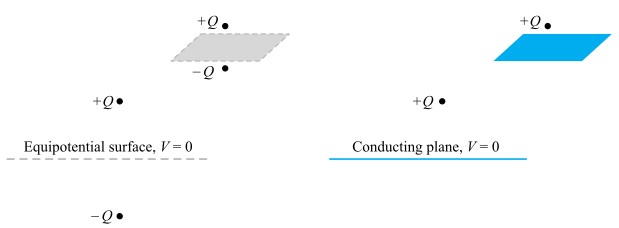
\includegraphics[scale=1]{image1.png}
\\
Un exemple de domaine connexe :
\\
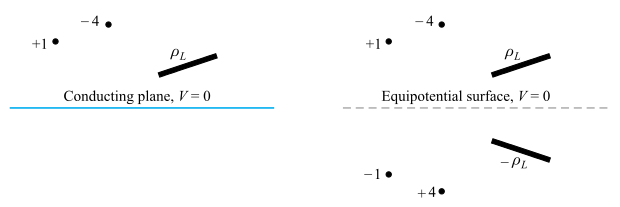
\includegraphics[scale=1]{image2.png}

\subsection{Démonstration constructive}

(C'est une démonstration qui explique comment calculer en plus de démontrer)

On considère dans l'espace de $\mathbb{R}^3$, un point $P$ de coordonnées $P_0 = (x_0,y_0,z_0) $  et $P = (x,y,z)$

\[P_0, P \in D \text{ ouvert et connexe }\]

On définit $\Phi$ tel que

\[\Phi (x,y,z ) =\int_C F\cdot \dif r \]
où C est une courbe reliant $P_0$ à $P$.

On a utilisé le fait que le domaine est connexe et qu'il y a indépendance des chemins.

On va montrer que \[\nabla \Phi = F \Longleftrightarrow F \text{ conserv.} \]

\[\frac{\partial \Phi}{\partial x} \overset{?}{=} F_1 (x,y,z) \]

On peut trouver un point $P' = ( x_1,y,z)$ tel que $x_1 < x$ est dans le domaine. On est certain de le trouver comme le domaine est ouvert.

\includegraphics[scale=0.7]{image4.png}

\[C=C_1+C_2\]
\[\Phi (x,y,z) = \int_{C_1} F + \int_{C_2} F\]

On trouve que $\int_{C_1} F$ ne dépend pas de x. Donc $\frac{\partial I_1}{\partial x }=0$

\[x_1\leq t \leq x \]
\[r(t) = t \xunit +y\yunit + z \zunit \]
\[\dif r = \frac{\dif r}{\dif t}\dif t = (\dif t)\xunit\]

On a donc

\[I_C = \int_{x_1}^x (F\cdot i)dt = \int_{x_1}^x F_1 \dif t\] avec $F_1 = F_1 ( t,y,z )$

On vient de montrer que

\[\frac{\partial I_2	}{\partial x} = F_1 = \frac{\partial \Phi}{\partial x}\]


\begin{mytheo}

\textbf{À connaître}

Soit $D$ ouvert connexe de $\mathbb{R}^n$ et $F$ champ de vecteurs défini dans $D$. Il y a \textbf{équivalence} des trois énoncés suivants.

\begin{itemize}
\item $F$ est conservatif sur $D$, c'est-à-dire qu'il existe un potentiel scalaire $\Phi$ tel que $F=\nabla \Phi $ dans $D$;
\item $\oint_C F =0 \forall $ courbe fermée de $D$;
\item $\forall P_0,P_1$ dans $D$, $\forall$ chemin $C$ reliant $P_0$ et $P_1$ dans $D$,
\end{itemize}
\[\int_C D \text{ a une valeure identique ( indépendance de chemin ) }\]

\end{mytheo}

\begin{mytheo}[Théorème de Poincaré]

Connaissant $F$, puis-je facilement décider si $F$ est (ou non) conservative ? (Sans essayer de trouver un potentiel $\Phi$ ni essayer de trouver une infinité de chemins).

Nous verrons plus loin que pour D simplement connexe, on peut ajouter un 4\ieme{} énoncé.

$$\frac{\partial F_i}{\partial x_j} = \frac{\partial F_j}{\partial x_i}$$

Ce théorème est applicable uniquement si le domaine est simplement connexe.
\end{mytheo}

\begin{mydef}
$D$ simplement connexe ssi connexe et toute courbe fermée qui ne s'intersecte pas peut être  transformée continument en un point de $D$ sans quitter $D$.
\end{mydef}

Par exemple :

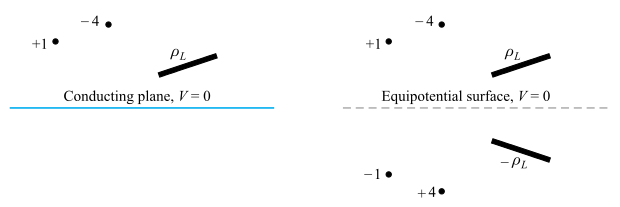
\includegraphics[scale=0.7]{image2.png}\\
n'est pas simplement connexe.
La fonction $ \Phi =xy^2 $  est le potentiel $F=y^2\xunit +2xy\yunit$ (par définition, c'est un champ de vecteur conservatif.)

$F= y\xunit-x\yunit$, calculons, $\frac{\partial F_1}{\partial y} = 1 \neq \frac{\partial F_2}{\partial x} = -1$. En effet, pour qu'un champ de vecteurs soit conservatif, il faut que ces deux dérivées partielles soient égales.

Pour utiliser le Théorème de Poincaré, on doit d'abord vérifier que les hypothèses sont vérifiées.

\section{Le flux d'un champ de vecteur à travers une surface}

cf.~\cite{adams2013calculus} section~15.6

C'est une intégrale de surface de la composante normale à une surface d'un champ de vecteurs.

\subsection{Introduction}
 Surface orientée\\
 \includegraphics[scale=0.6]{image5.png}

 Le côté positif de la surface est le côté du vecteur normal tandis que le côté négatif, c'est l'autre.

 Par convention, l'orientation d'une surface induit une orientation particulière des bords de la surface (s'ils existent).

 La règle est la suivante : on se met sur la face positive de $S$ et on marche le long du bord $C$ en laissant $S$ à gauche, ce qui définit l'orientation positive de $C$.

 \includegraphics[scale=0.7]{image6.png}
 \\

 La face positive est au-dessus et la face négative est en-dessous. Par convention, les flèches représentent le sens de parcours positif.

 Voir ces exemples :

 \includegraphics[scale=0.6]{image7.png}\\
 \includegraphics[scale=0.6]{image8.png}

 \subsection{Flux d'un champ vectoriel à travers une surface}

 On souhaite connaître la vitesse d'un cours d'eau à un endroit donné. On va placer une surface S fictive.\\

 \includegraphics[scale=0.5]{image9.png} % Image 15.29
\\ On cherche le volume du cylindre. On pose $\rho \equiv 1$

 \[Vol = \norm{V}\dif t \cos \Theta \dif S\]

 avec $\norm{V}\dif t \cos \Theta = V\cdot \hat N \dif S$


 Par unité de temps, la quantité de fluide qui passe à travers $\dif S$ est donc \[V(P) \cdot \hat N(P) \dif S\]

 \[\int_S \text{flux } \dif S = \text{ flux total de matière à travers S.}\]

 \begin{mydef}
 Le flux d'un champ de vecteurs $F$ à travers une surface orientée S est donné par\[\int_S F \cdot \hat N \dif S = \int_S F \cdot \vv{\dif S}\]

 et $F \cdot \hat N$ est la composante normale à $S$ de $F$ avec $\vv{\dif S} = \hat N \dif S$ élément de surface vectoriel.

 Notation : $\int_C F$
 \end{mydef}

\begin{myrem}

$S$ fermée (sphère) :  $ \oiint_S F\cdot \dif S$

\[\oint F\cdot \dif r\]

\end{myrem}

Exemple : $F = (x) \xunit + (y) \yunit+(z) \zunit$

Flux sortant du cylindre
\[\left\{
\begin{array}{c}
F=y^2\xunit+2xyjx^2+y^2\leqslant a^2 \\ % FIXME je ne sais vraiment pas ce qui était sensé être écrit
-h\leqslant z \leqslant h
\end{array}
\right.\]


La surface totale $S$ : dessus + dessous + coté.

\includegraphics[scale=0.5]{image10.png}

\[\int_S F\cdot \dif S = \Sigma\text{flux}\]

On calcule sur chacune des faces.

\begin{enumerate}
  \item
    $z = +h$; $\hat N = \zunit$ et  $\dif S= r\dif\Theta \dif r$

    \[\int_{top}F\cdot \hat N \dif S = \int_O^{2\pi} d\Theta \int_0^a h r \dif r = \pi a^2 h\]

  \item $z = -h$; $\hat N = -k \Rightarrow =\pi a^2 h $

  \item coordonnées cylindriques

    \[-h \leq z\leq h \] et aussi
    \[0\leq \Theta \leq 2 \pi\]

    $\dif S = a\dif \Theta \dif z$

    \[\vec{F} = (a\cos\Theta ) \xunit +(a\sin\Theta ) \yunit + z \zunit  \]

    \[\hat N = (\cos\Theta ) \xunit +a\sin\Theta ) \yunit\Leftrightarrow \vec F \hat N \dif S = a^2\dif \Theta \dif z\]
    \[\int_0^{2\pi} \dif \Theta \int_{-h}^{+h} a^2 \dif z = 4\pi a^2 h\]

\end{enumerate}

Le flux total vaut donc la somme de (1), (2) et (3) $= 6 \pi a^2 h $

\fbox{
\begin{minipage}{10cm}
\textbf{Formule à connaître \# 5}

Règle de calcul


$r(u,v)$ de $S$ avec $(u,v) \in D \subset \mathbb{R}^2$

On a vu que :
\begin{itemize}
\item
$n=\frac{\partial r}{\partial u } \times \frac{\partial r}{\partial v }$

normal à $S$ (Par définition du produit vectoriel)

\[\hat N = \pm \frac{n}{\norm{n}}\]
le $\pm$ dépend de notre choix d'orientation de S.
\item
\[ \dif S = \norm{n} \dif u\dif v \]
\end{itemize}

On a donc
\[ \vv{\dif S} = \hat N \dif S = \pm\frac{n}{\norm{n}}\dif u\dif v = \pm
n \dif u \dif v \]

et finalement, $F=F_1(x,y,z)\xunit+F_2(x,y,z)\yunit+F_3(x,y,z)\zunit$

Le flux de $F$ à travers $S$ est donné par

\[\int_S F\cdot \dif S = \pm \int_D F\cdot \left(\frac{\partial r}{\partial u } \times \frac{\partial r}{\partial v } \right) \dif u\dif v\]


 Cette formule nous permet de calculer l'intégrale d'un champ vectoriel à travers une surface.
\end{minipage} }

\begin{align*}
\text{Flux} &= \pm \int \left(F_1( x(u,v),y(u,v),z(u,v) )\frac{\partial(y,z)}{\partial (u,v)} \right. \\
&+ F_2( x(u,v),y(u,v),z(u,v))\frac{\partial(z,x)}{\partial (u,v)} \\
&+ \left. F_3( x(u,v),y(u,v),z(u,v))\frac{\partial(x,y)}{\partial (u,v)}\right) \dif u\dif v \\
\end{align*}

avec par exemple

\[\frac{\partial(z,x)}{\partial (u,v)}=\frac{\partial z}{\partial u}\frac{\partial x}{\partial v}-\frac{\partial z}{\partial v}\frac{\partial x}{\partial u}\]

et \[\vec r (u,v) = x(u,v)\xunit +y(u,v)\yunit +z(u,v)\zunit \]
